\documentclass[]{article}
\pagenumbering{gobble}
\usepackage[a3paper, total={6in, 8in}]{geometry}

\usepackage{pgfplots}
\usepackage{tcolorbox}
\usepackage{circuitikz}
\usepackage{amsmath}
\usepackage{pgfplotstable}
\pgfplotsset{compat=1.18}

\usepackage{tikz}
\usetikzlibrary{automata, positioning, arrows, calc}

\tikzset{
	->,
	>=stealth,
	node distance=3cm,
	every state/.style={thick, fill=gray!10},
	initial text=$ $,
}

%opening
\title{Paper assignement 2: Xurl state machine}
\author{Gabriel PEREIRA DE CARVALHO}
\date{Last modification: \today}

\begin{document}
	
	\maketitle
	
	\begin{figure}
		\centering
		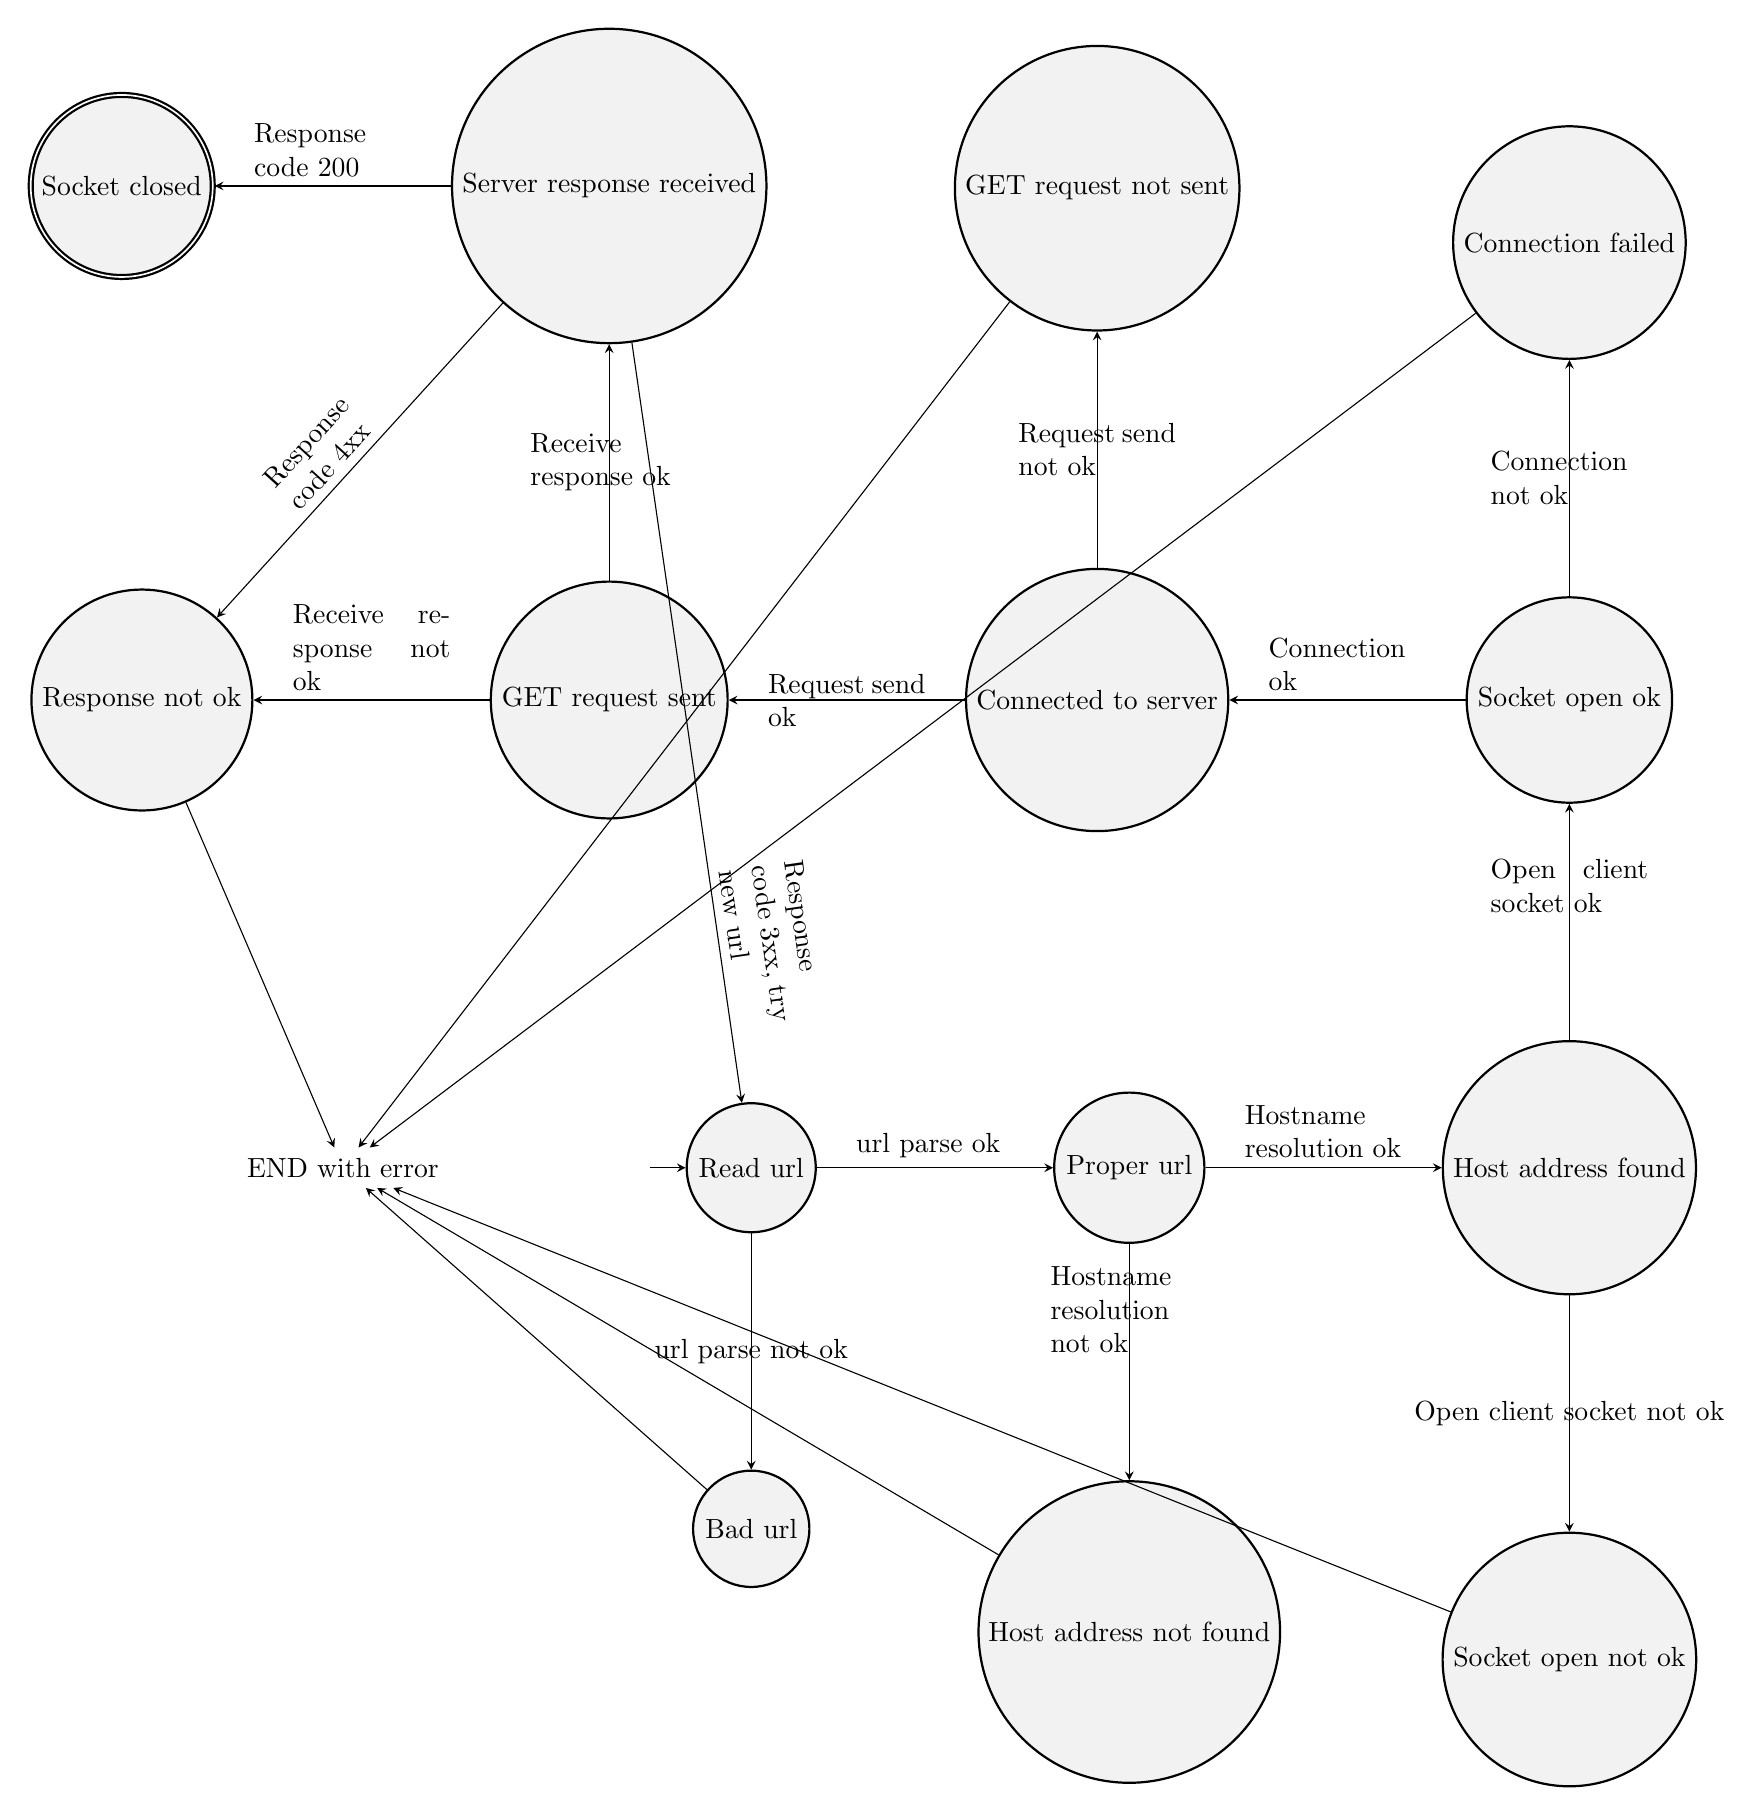
\begin{tikzpicture}
			\node [state, initial] (START) {Read url};
			\node [accepting, left=of START] (END) {END with error};
			\node [state, below=of START] (BADurl) {Bad url};
			\node [state, right=of START] (GOODurl) {Proper url};
			\node [state, right=of GOODurl] (HOSTfound) {Host address found};
			\node [state, below=of GOODurl] (HOSTunfound) {Host address not found};
			\node [state, above=of HOSTfound] (SOCKETopen) {Socket open ok};
			\node [state, below=of HOSTfound] (SOCKETunopen) {Socket open not ok};
			\node [state, left=of SOCKETopen] (CONNECTok) {Connected to server};
			\node [state, above=of SOCKETopen] (CONNECTunok) {Connection failed};
			\node [state, left=of CONNECTok] (SENDok) {GET request sent};
			\node [state, above=of CONNECTok] (SENDunok) {GET request not sent};
			\node [state, above=of SENDok] (RESPONSEok) {Server response received};
			\node [state, left=of SENDok] (RESPONSEunok) {Response not ok};
			\node [state, accepting, left=of RESPONSEok] (OK) {Socket closed};
			
			\draw (START) edge[] node{url parse not ok} (BADurl);
			\draw (START) edge[] node[above]{\parbox{2cm}{url parse ok}} (GOODurl);
			\draw (GOODurl) edge[] node[above]{\parbox{2cm}{Hostname resolution ok}} (HOSTfound);
			\draw (GOODurl) edge[] node[above]{\parbox{2cm}{Hostname resolution not ok}} (HOSTunfound);
			\draw (HOSTfound) edge[] node[above]{\parbox{2cm}{Open client socket ok}} (SOCKETopen);
			\draw (HOSTfound) edge[] node[]{Open client socket not ok} (SOCKETunopen);
			\draw (SOCKETopen) edge[] node[above]{\parbox{2cm}{Connection ok}} (CONNECTok);
			\draw (SOCKETopen) edge[] node[]{\parbox{2cm}{Connection not ok}} (CONNECTunok);
			\draw (CONNECTok) edge[] node[]{\parbox{2cm}{Request send ok}} (SENDok);
			\draw (CONNECTok) edge[] node[]{\parbox{2cm}{Request send not ok}} (SENDunok);
			\draw (SENDok) edge[] node[]{\parbox{2cm}{Receive response ok}} (RESPONSEok);
			\draw (SENDok) edge[] node[above]{\parbox{2cm}{Receive response not ok}} (RESPONSEunok);
			\draw (RESPONSEok) edge[] node[above]{\parbox{2cm}{Response code 200}} (OK);
			\draw (RESPONSEok) edge[] node[sloped, above]{\parbox{2cm}{Response code 4xx}} (RESPONSEunok);
			\draw (RESPONSEok) edge[] node[pos=0.8, sloped, above]{\parbox{2cm}{Response code 3xx, try new url}} (START);
			
			
			\draw (BADurl) edge[] node[]{} (END);
			\draw (HOSTunfound) edge[] node[]{} (END);
			\draw (SOCKETunopen) edge[] node[]{} (END);
			\draw (CONNECTunok) edge[] node[]{} (END);
			\draw (SENDunok) edge[] node[]{} (END);
			\draw (RESPONSEunok) edge[] node[]{} (END);
			
		\end{tikzpicture}
	\end{figure}
	
\end{document}